\part{Validation}

\chapter{Solution validation}

\section {Data model}

The model designed for the Observatory project represented in figure~\ref{fig:datamodel-obsproject} is a simplification of the ALMA Project Data Model summarized in section~\ref{sec:apdm} and it is the model used in the ALMA's Dynamic Scheduling Algorithm briefly described in section~\ref{sec:alma-dsa}.

The most relevant parts are: 
\begin{description}
\item[bla1] \hfill \\
Description of bla1
\end{description}

\begin{figure}[]	
\begin{center}
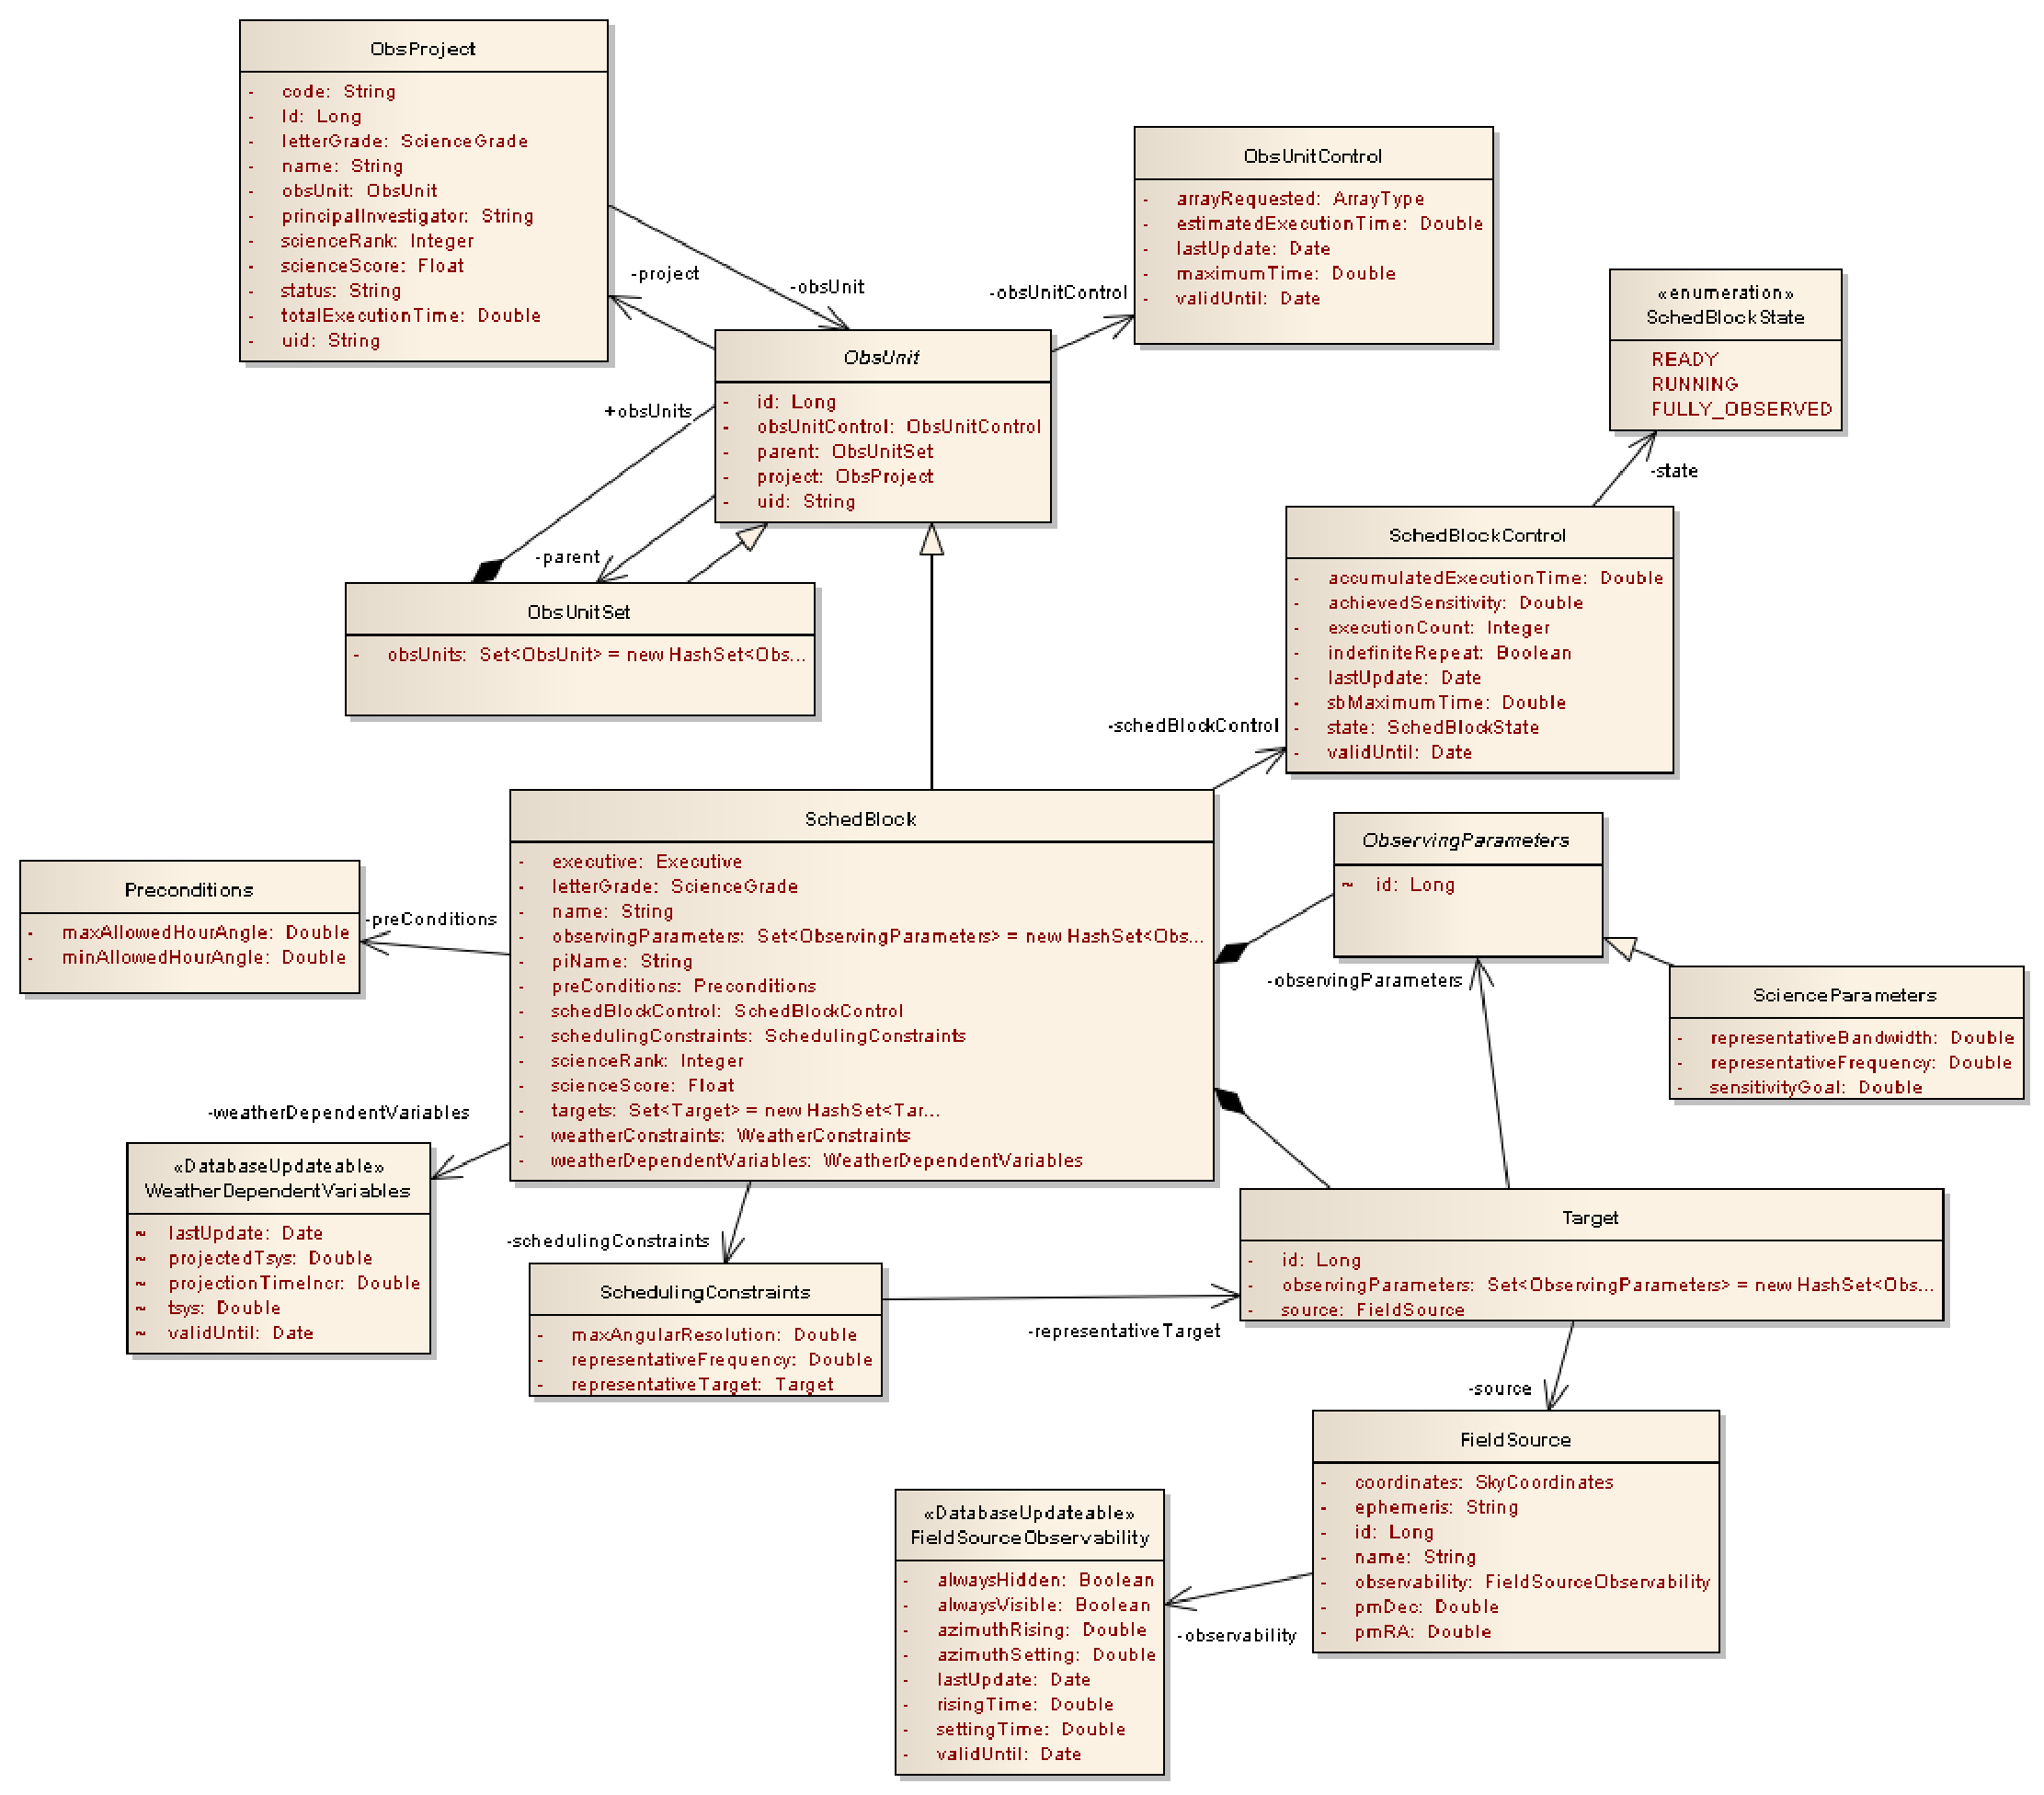
\includegraphics[width=1.15\textwidth]{images/ObsProject}
\caption{Observation Project data model}
\end{center}
\label{fig:datamodel-obsproject}
\end{figure}

The model designed for handle the observatory instrumentation is represented in figure~\ref{fig:datamodel-observatory}

\begin{figure}[]	
\begin{center}
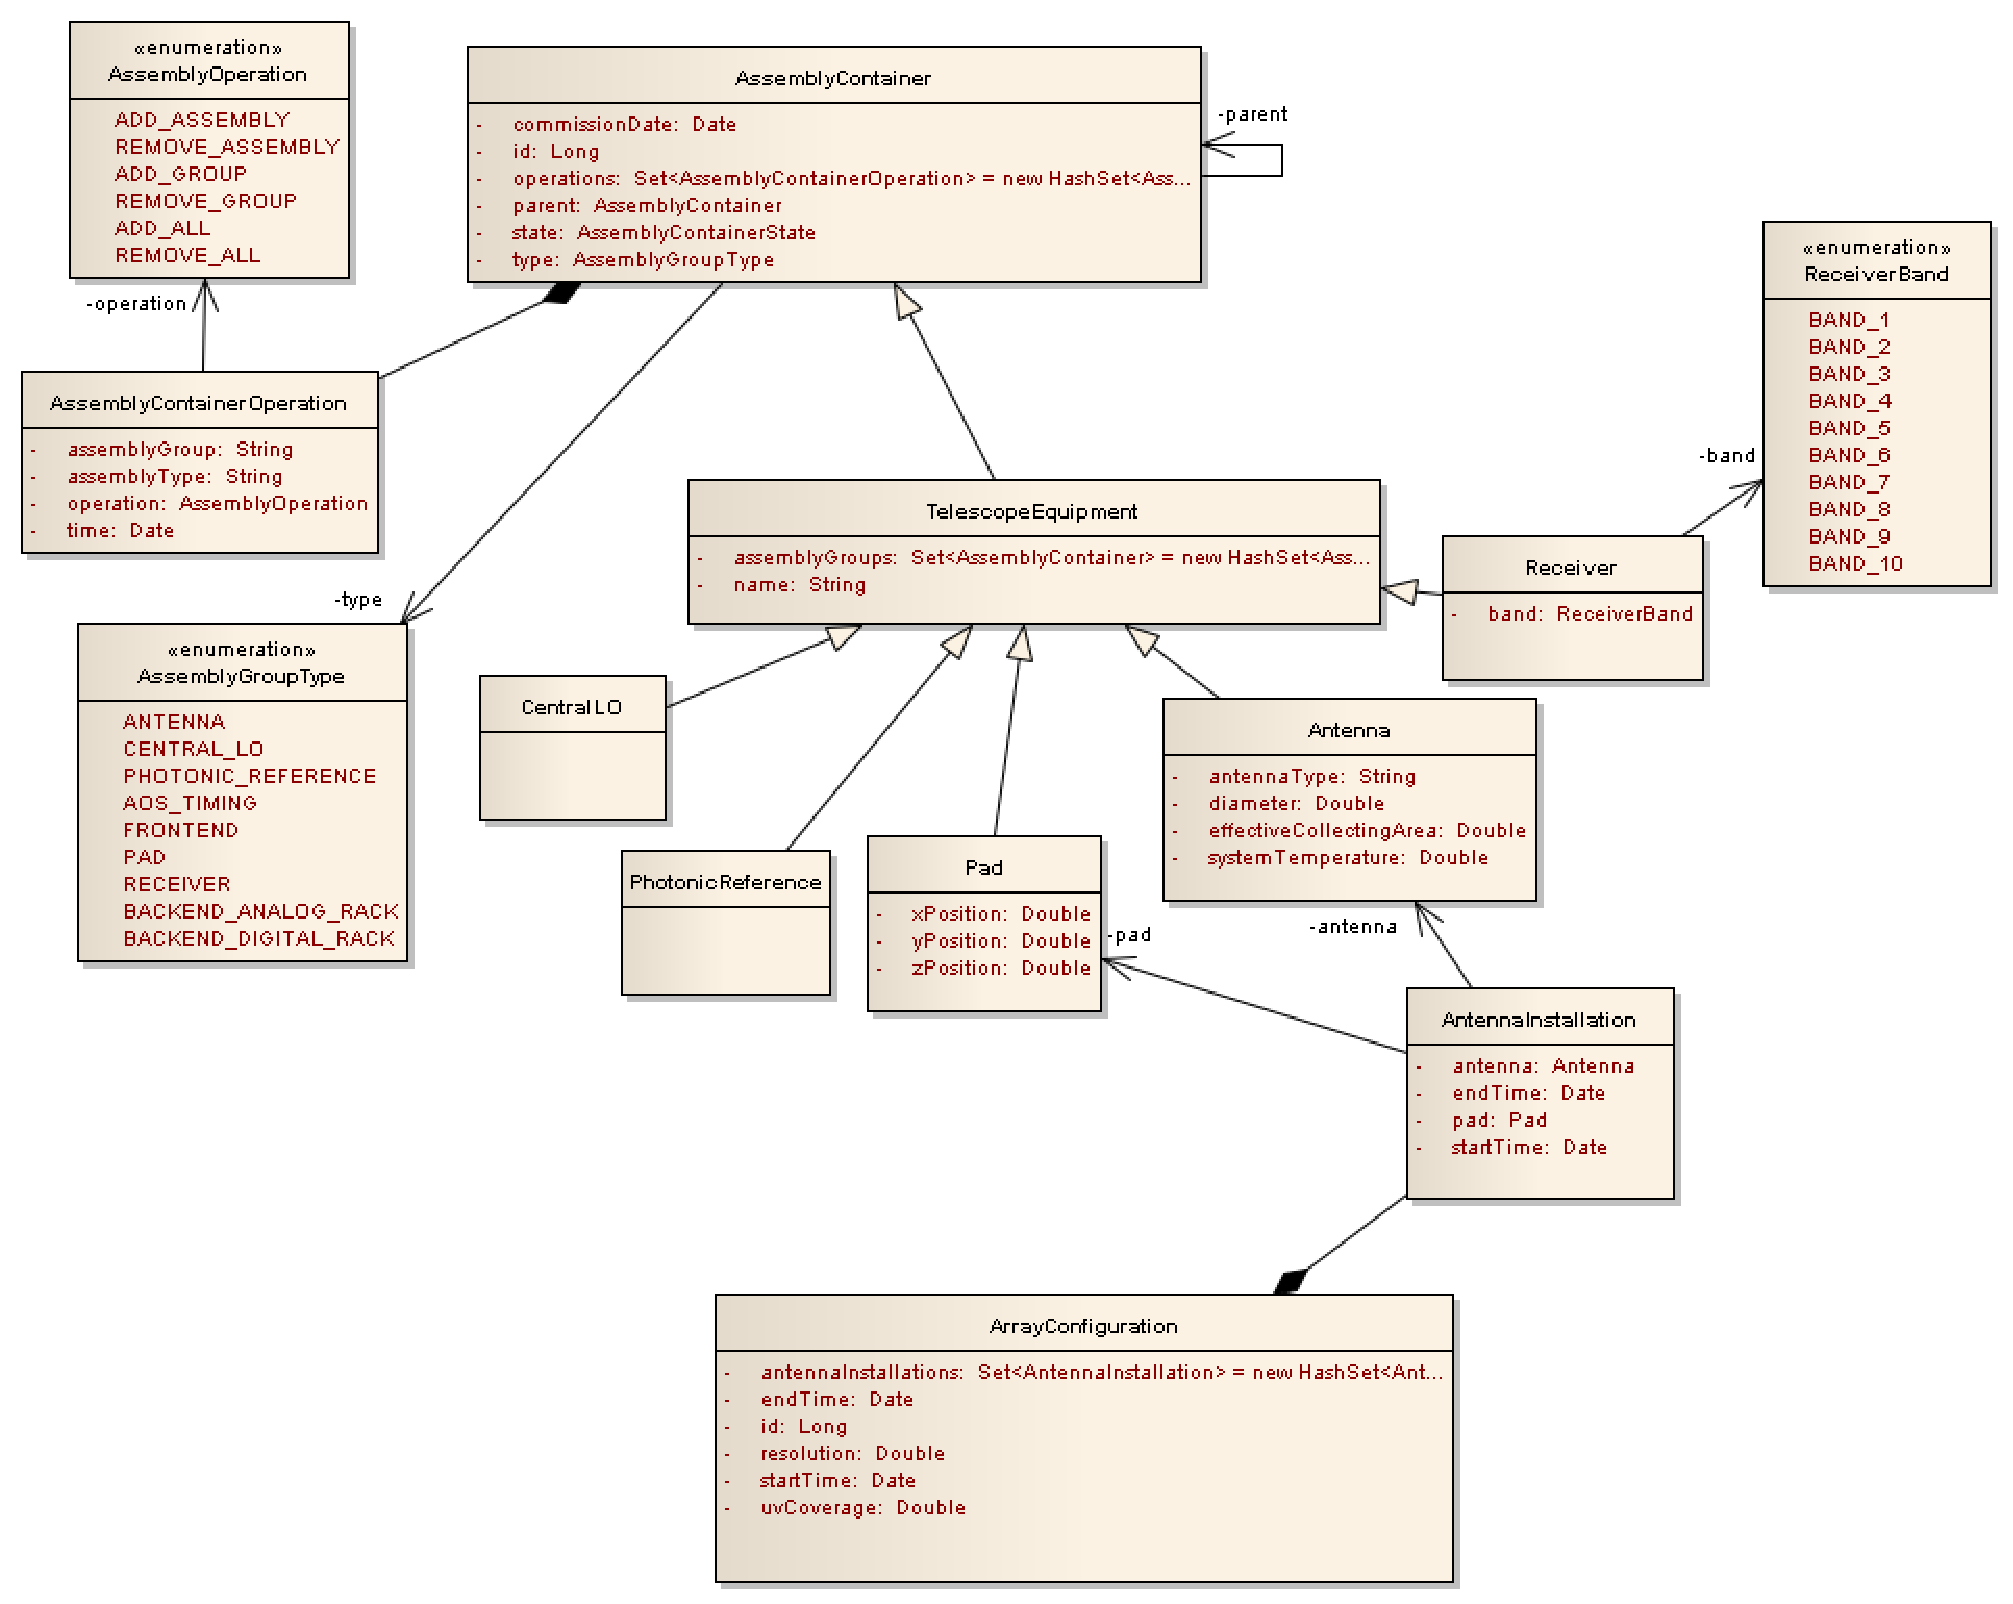
\includegraphics[width=\textwidth]{images/Observatory}
\caption{Observatory instrumentation data model}
\end{center}
\label{fig:datamodel-observatory}
\end{figure}

The model designed for handle the Executive information and the observing season is represented in figure~\ref{fig:datamodel-executive}

\begin{figure}[]	
\begin{center}
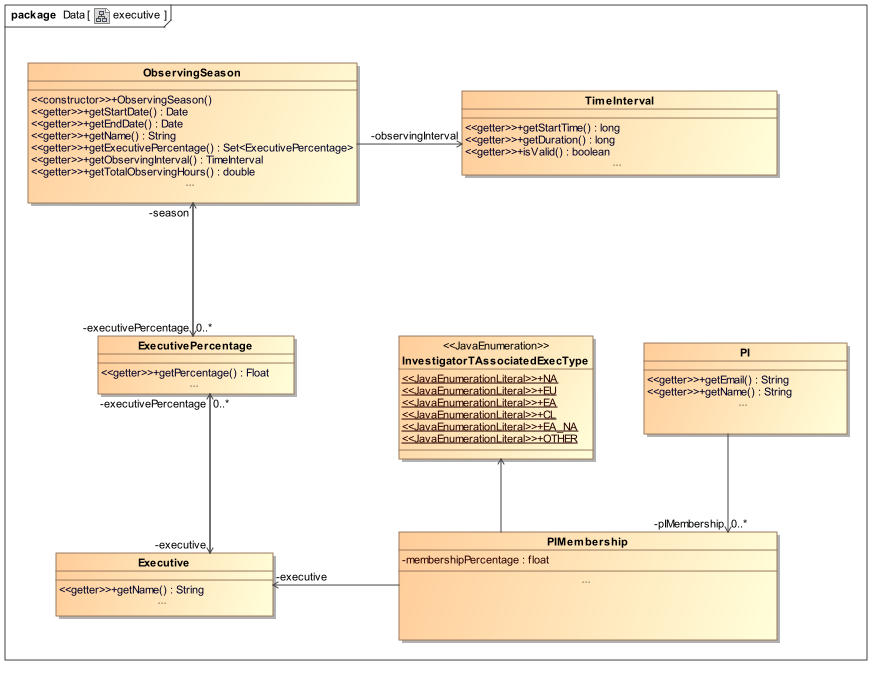
\includegraphics[width=\textwidth]{images/Executive}
\caption{Executive and observing season data model}
\end{center}
\label{fig:datamodel-executive}
\end{figure}

The model designed for handle the weather is represented in figure~\ref{fig:datamodel-weather}

\begin{figure}[]	
\begin{center}
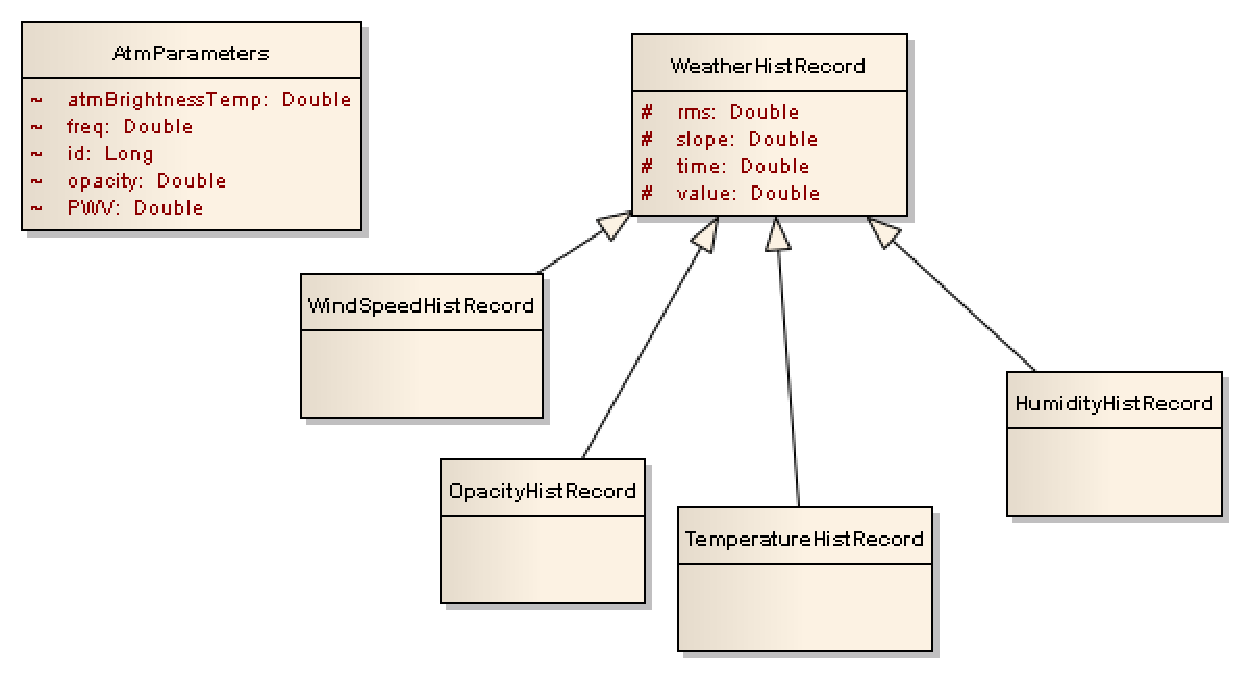
\includegraphics[width=\textwidth]{images/Weather}
\caption{Executive and observing season data model}
\end{center}
\label{fig:datamodel-weather}
\end{figure}

\section {Simulation}

\begin{figure}[]	
\begin{center}
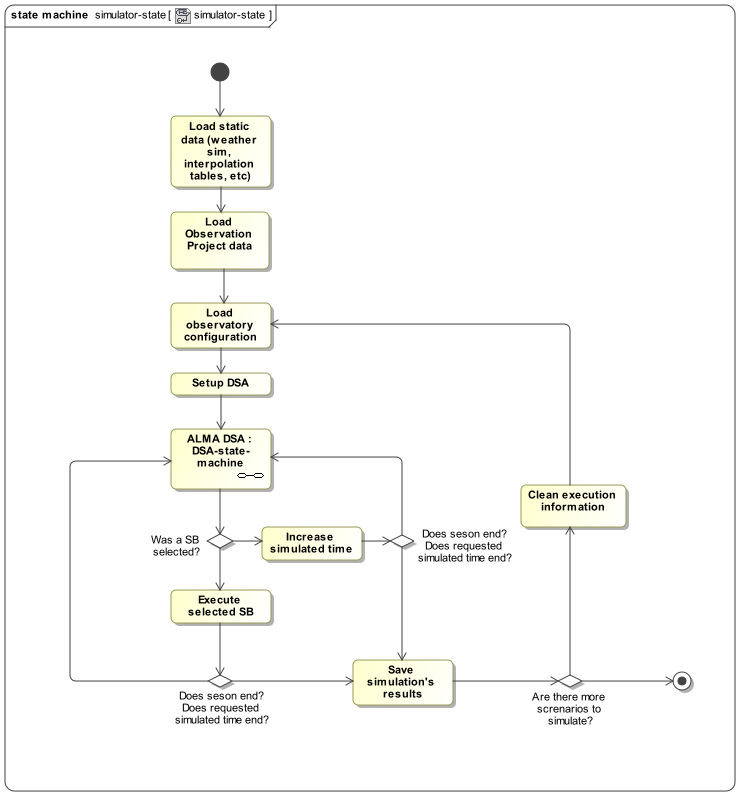
\includegraphics[width=\textwidth]{images/simulator-state-machine}
\caption{ALMA simulator's state machine}
\end{center}
\label{fig:sim-state-machine}
\end{figure}

\section {Algorithm implementation}

\section {Input Observation projects}

\begin{table}
\begin{center}
\begin{tabular}{|c|c|c|c|}
\hline
Configuration name & Array type & Min. Baseline $[m]$ & Max. Baseline $[m]$\\
\hline
C34-1 & $12\,[m]$ & $14.2$ & $165.6$ \\
\hline
C34-2 & $12\,[m]$ & $14.1$ & $303.6$ \\
\hline
C34-3 & $12\,[m]$ & $20.6$ & $442.7$ \\
\hline
C34-4 & $12\,[m]$ & $20.6$ & $558.2$ \\
\hline
C34-5 & $12\,[m]$ & $25.8$ & $820.2$ \\
\hline
C34-6 & $12\,[m]$ & $40.6$ & $1091.0$ \\
\hline
C34-7 & $12\,[m]$ & $40.6$ & $1507.9$ \\
\hline
7m    & $7\,[m]$  & $8.9$  & $32.1$ \\
\hline
TP    & $TP$      & $-$    & $-$ \\
\hline
\end{tabular}
\end{center}
\caption{Array configurations provided as input for the algorithms}
\label{table:input-array-configs}
\end{table}

\begin{table}
\begin{center}
\begin{tabular}{|c|c|c|c|}
\hline
Grade & Executive & Time Requested $[h]$ & Number of Scheduling Blocks \\ \hline
A &	CL		& 12.0  & 2 \\ \hline
A &	EA		& 36.0  & 13 \\ \hline
A &	EA/NA	& 6.0   & 3 \\ \hline
A & EU      & 112.0 & 31 \\ \hline 
A &	NA		& 114.0	& 31 \\ \hline
A & OTHER	& 0		& 0 \\ \hline
B  & CL 	& 160.0		& 48  \\ \hline
B  & EA     & 438.0     & 145 \\ \hline
B  & EA/NA  & 106.0     & 30  \\ \hline
B  & EU     & 828.0     & 280 \\ \hline
B  & NA     & 1024.0    & 344 \\ \hline
B  & OTHER  & 40.0      & 19  \\ \hline
C  & CL     & 130.0     & 50  \\ \hline
C  & EA     & 246.0     & 65  \\ \hline
C  & EA/NA  & 52.0      & 23  \\ \hline
C  & EU     & 410.0     & 155 \\ \hline
C  & NA     & 556.0     & 196 \\ \hline
C  & OTHER  & 34.0      & 13  \\ \hline
\end{tabular}
\end{center}
\caption{Requested time for $12m$ array configurations}
\label{table:requested-time-12m}
\end{table}

\begin{table}
\begin{center}
\begin{tabular}{|c|c|c|c|}
\hline
Grade & Executive & Time Requested $[h]$ & Number of Scheduling Blocks \\ \hline
A &	CL		& 0  & 0 \\ \hline
A &	EA		& 24.0  & 1 \\ \hline
A &	EA/NA	& 6.0   & 12 \\ \hline
A & EU      & 12.0 & 1 \\ \hline 
A &	NA		& 16.0 & 2 \\ \hline
A & OTHER	& 0		& 0 \\ \hline
B  & CL 	& 16.0		& 1  \\ \hline
B  & EA     & 78.0     & 21 \\ \hline
B  & EA/NA  & 22.0     & 5  \\ \hline
B  & EU     & 168.0     & 41 \\ \hline
B  & NA     & 182.0    & 29 \\ \hline
B  & OTHER  & 0.0      & 0  \\ \hline
C  & CL     & 38.0     & 2  \\ \hline
C  & EA     & 46.0     & 12  \\ \hline
C  & EA/NA  & 36.0      & 9  \\ \hline
C  & EU     & 5800     & 7 \\ \hline
C  & NA     & 556.0     & 196 \\ \hline
C  & OTHER  & 72.0      & 12  \\ \hline
\end{tabular}
\end{center}
\caption{Requested time for $7m$ array configurations}
\label{table:requested-time-7m}
\end{table}

\begin{table}
\begin{center}
\begin{tabular}{|c|c|c|c|}
\hline
Grade & Executive & Time Requested $[h]$ & Number of Scheduling Blocks \\ \hline
A &	CL		& 0  & 0 \\ \hline
A &	EA		& 28.0  & 1 \\ \hline
A &	EA/NA	& 208.0   & 2 \\ \hline
A & EU      & 132.0 & 1 \\ \hline 
A &	NA		& 112.0 & 2 \\ \hline
A & OTHER	& 0		& 0 \\ \hline
B  & CL 	& 28.0		& 1  \\ \hline
B  & EA     & 1852.0     & 21 \\ \hline
B  & EA/NA  & 752.0     & 5  \\ \hline
B  & EU     & 922.0     & 41 \\ \hline
B  & NA     & 1792.0    & 29 \\ \hline
B  & OTHER  & 0.0      & 0  \\ \hline
C  & CL     & 52.0     & 2  \\ \hline
C  & EA     & 1250.0     & 12  \\ \hline
C  & EA/NA  & 824.0      & 9  \\ \hline
C  & EU     & 368.0     & 7 \\ \hline
C  & NA     & 78.0     & 12 \\ \hline
C  & OTHER  & 2.0      & 1  \\ \hline
\end{tabular}
\end{center}
\caption{Requested time for $TP$ array configurations}
\label{table:requested-time-tp}
\end{table}

\begin{figure}
        \centering
        \begin{subfigure}[b]{0.49\textwidth}
                \includegraphics[width=\textwidth]{images/c34-1_sources}
                \caption{C34-1} 
        \end{subfigure} 
        ~ %
%
        \begin{subfigure}[b]{0.49\textwidth}
                \includegraphics[width=\textwidth]{images/c34-2_sources}
                \caption{C34-2}
        \end{subfigure}

        \begin{subfigure}[b]{0.49\textwidth}
                \includegraphics[width=\textwidth]{images/c34-3_sources}
                \caption{C34-3}
        \end{subfigure}
        ~ 
        \begin{subfigure}[b]{0.49\textwidth}
                \includegraphics[width=\textwidth]{images/c34-4_sources}
                \caption{C34-4}
        \end{subfigure}% 
        
        \begin{subfigure}[b]{0.49\textwidth}
                \includegraphics[width=\textwidth]{images/c34-5_sources}
                \caption{C34-5}
        \end{subfigure}
        ~
        \begin{subfigure}[b]{0.49\textwidth}
                \includegraphics[width=\textwidth]{images/c34-6_sources}
                \caption{C34-6}
        \end{subfigure}
        
        \begin{subfigure}[b]{0.49\textwidth}
                \includegraphics[width=\textwidth]{images/c34-7_sources}
                \caption{C34-7}
        \end{subfigure}           
          
        \caption{Visibility of Scheduling Blocks for $12\,[m]$ Array Configurations}
        \label{fig:results-sb-critical-set}
\end{figure}